\cleardoublepage
\chapter{Introduction: Who should fear the Robot Apocolypse}

The news and popular culture want us to fear the robot apocolypse.  Newspapers warn us that robots are coming for our jobs, and science fiction claims that the robots are coming for our lives.  At the same time, researchers building artificial intelligence are heralding their sucesses at Go~\cite{silver-16}, Starcraft~\cite{vinyals2017starcraft}, and \series{Jeopardy!}~\cite{ferruci-10} a revolution is around the corner.

\begin{marginfigure}%
  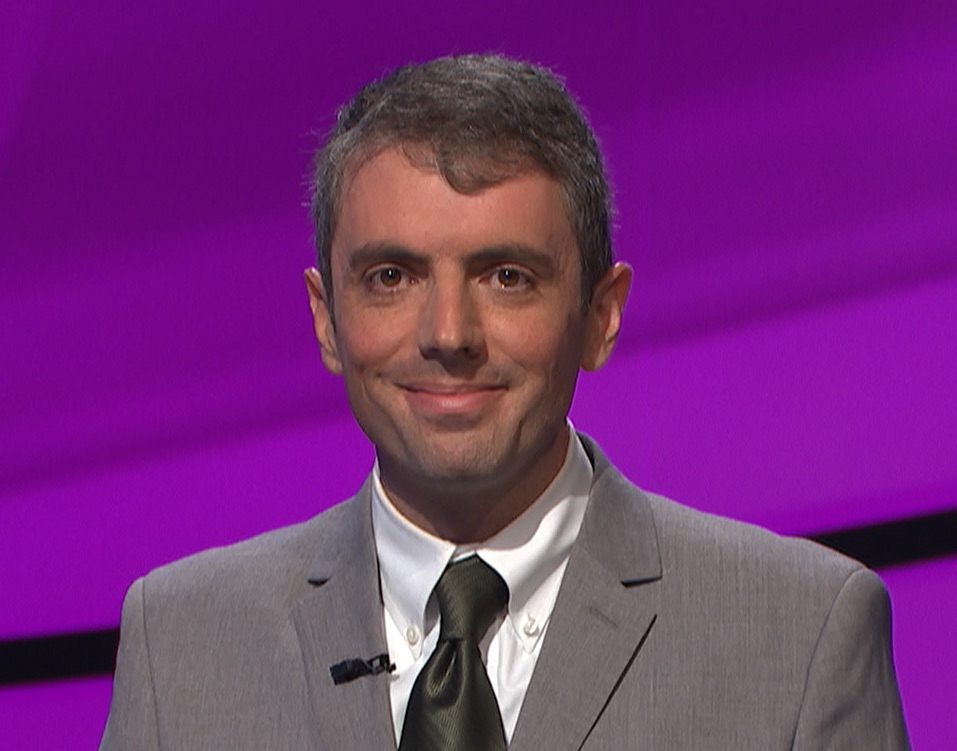
\includegraphics[width=\linewidth]{jbg}
  \caption{\href{http://boydgraber.org}{Jordan Boyd-Graber} is an associate professor at the University of Maryland who researches how computers can learn from humans and compete with humans.  You can watch his trivia playing robots \href{http://qanta.org/home/past-events}{take on humans on YouTube}.}
  \label{fig:marginfig}
\end{marginfigure}

\begin{marginfigure}%
  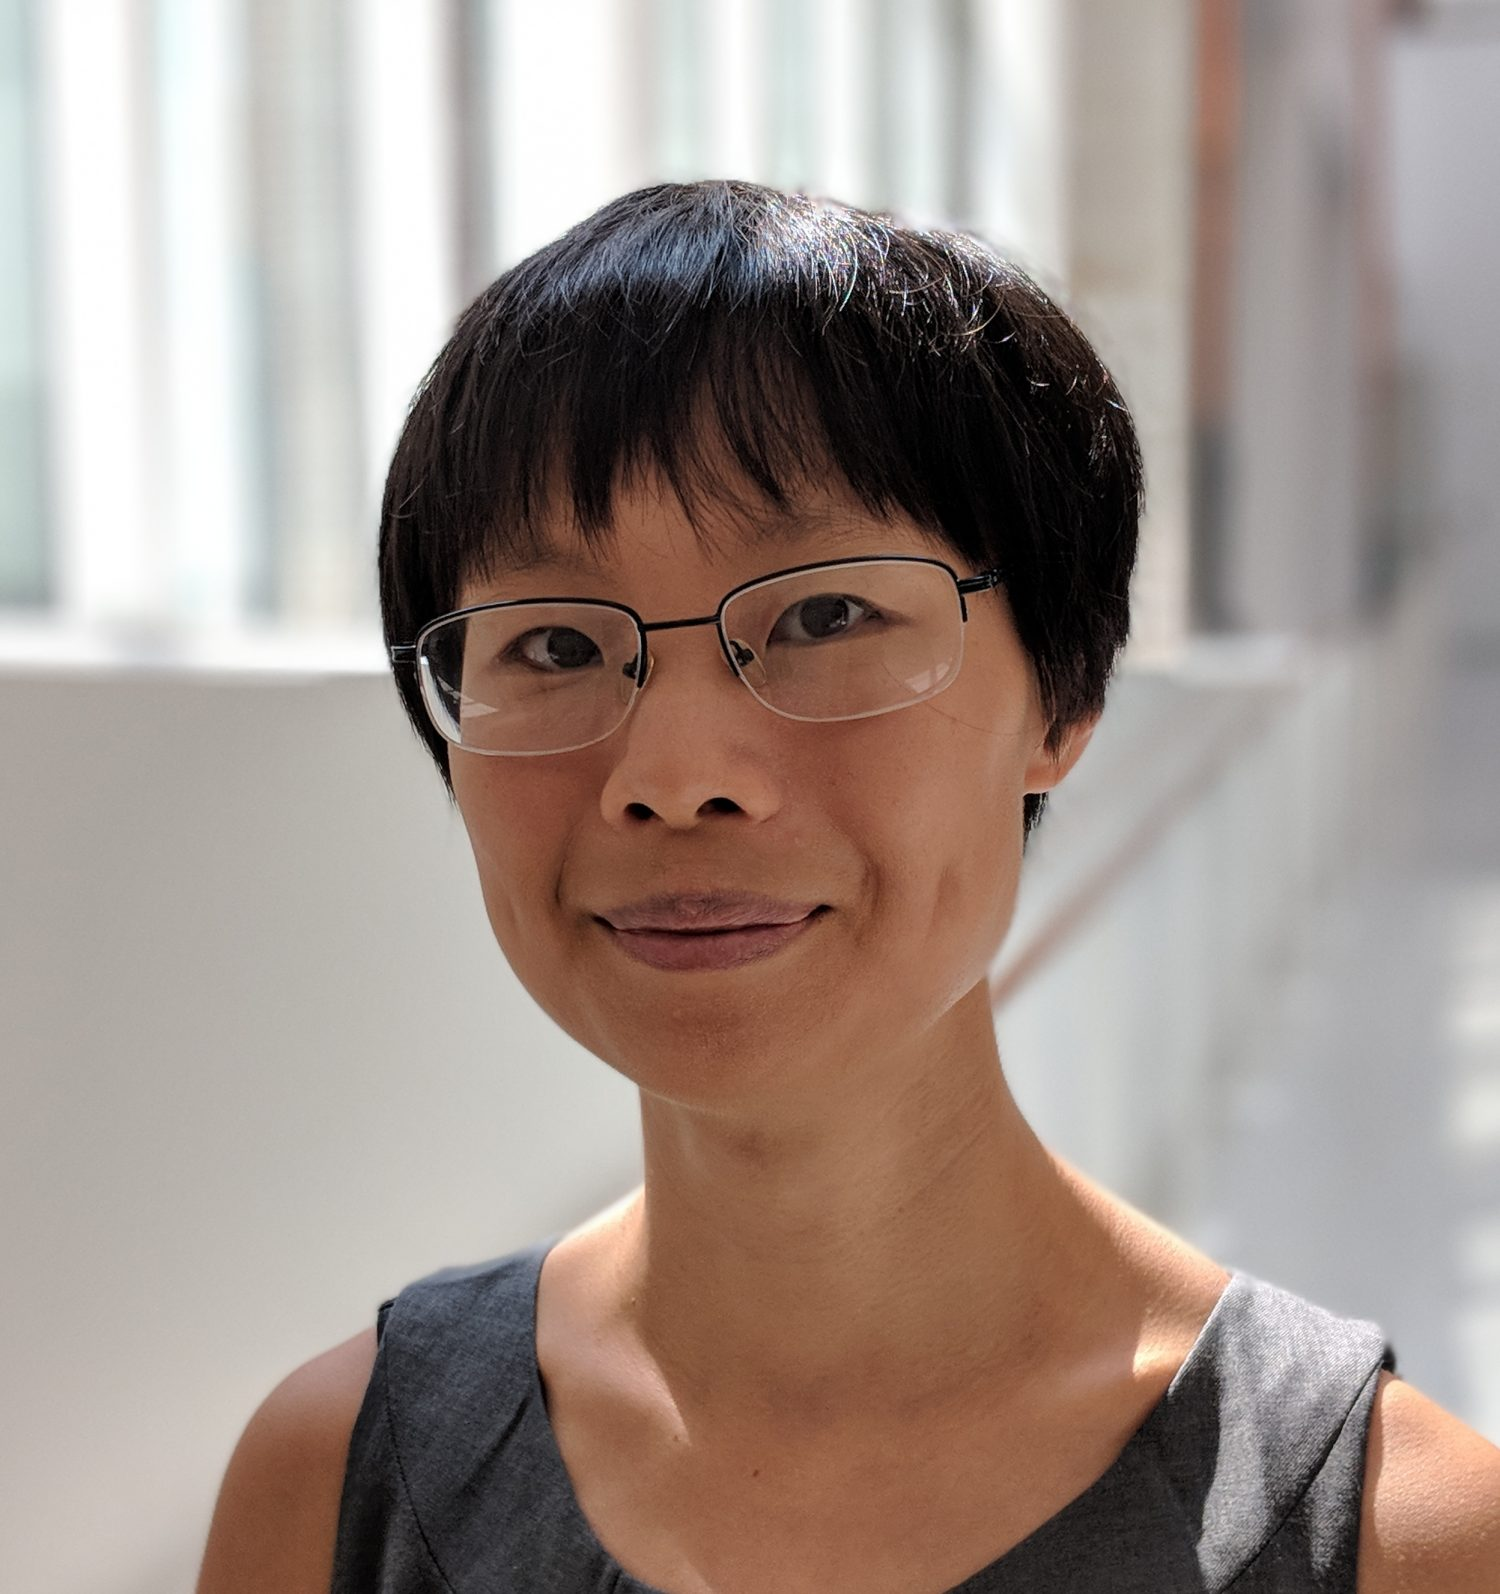
\includegraphics[width=\linewidth]{ziy}
  \caption{\href{http://www.ireneying.net/}{Z. Irene Ying} is a science writer who publishes science fiction as \href{http://www.windupdreams.net/}{Kara Lee}.}
  \label{fig:marginfig}
\end{marginfigure}

This book aims to bring together some of these threads into a coherent
narrative building on our experience as a science writer (Z. Irene
Ying) and an artifical intelligence researcher (Jordan Boyd-Graber).
We\footnote{At the risk of sowing confusion, we use ``we'' in this
chapter (first person), Jordan will use ``I'' in following essays, and
Irene will use the third person in the following stories.} agree that
there are lots of changes in artifcial intelligence and potential
changes to society, we do disagree with some of the dire predictions
we see from researchers, the news, and science fiction.

But nobody listens to our rants on Twitter or in the classroom, so we
decided to write a book.  It's not that we think that the future is
full sunshine, lollipops, and rainbows.\footnote{This titular opening
line from the song \song{Sunshine, Lollipops, and Rainbows} by Lesley
Gore that featured prominently in \series{The Simpsons}
episode \episode{Marge on the Lam} and the film \movie{Cloudy with a
Chance of Meatballs} is a good chance to show our typographic
conventions we'll use for our many pop culture references.}  We are as
scared as anybody else\dots we're just scared of different things, and
we'd like to use our background to try to get other people to be
afraid of the same things we are.

Science fiction typically emphasizes fiction over science (and rightly
so, it's more fun that way).  These stories focus on massive sudden
changes that uproot society overnight: a zombie virus destroys
civilization in twenty-eight days,\footnote{\movie{28 Days Later}, a
2002 British post-apocalyptic film where a genetically engineered
virus destroys England.} a military computer launches all of the
missiles to destroy the world,\footnote{SkyNet's plan for erradicating
humanity from the Terminator franchise.} or alien refugees overwhelm
society.\footnote{The 2009 film \movie{District 9} based
on \book{Alive in Joburg}} These sudden shocks to the system make for
good stories because we understand our culture \emph{as it is} and we,
as readers, can grapple with how our twenty minute in the future
selves would cope with these changes.

While technology does change society, these changes are typically slow.  While telephones frightened one generation, it took so long to figure out how to use them effectively that by the time they were integrated fully into society, the next generation had lived with the \emph{idea} of telephones so long that they were no longer viewed as an exestential threat.  The fear with artificial intelligence and robots is that progress is so quick that we won't have this comfortable buffer period\dots but for those in the trenches, progress feels achingly slow.  

Researchers focus on what works.  We spend years getting a system to answer trivia questions to work, so we want to show off what it's capable of.  We focus on how it's able to know that ``Roark's Drift'' is in South Africa and not how it answers every math question with ``six'' (true story).  We are still a long way from anything close to a child's intelligence, let alone something that would challenge humanity's supremacy.  

\section{How the Book is Structured}

We are not the only ones saying this; plenty of researchers warn of overselling the hype around machine intelligence.  However, these boring essays and conference presentations don't really stack up against a big-budget western with Anthony Hopkins creating sexy killbots.\footnote{\series{Westworld}, an HBO series about a western theme park populated by intelligent robots.}  We don't have that budget either,\footnote{However, if anyone, including Anthony Hopkins, would like to give us a big budget, a sound stage, or sexy killbots, we'd put them to good use.} but what we can do is create sci-fi stories that better comport with the realities of science fiction.

When people hear about the latest advance in artificial intelligence they often imagine how it will change their lives.  This book does the same thing\dots presenting a sseries of short stories about how aritifical intelligence can shape culture, politics, and the economy.  What is unique (or at least unusual) about this book it is shaped by an understanding of what machine learning research is doing.

Interleaved with each of these fictional extrapolations is a more scientifically oriented story that combines technical insights and the literature of the research community that drove some of the storytelling choices of the fictional chapters.  These chapters are more academic in tone (but hopefully a little more accessible and playful than the turgid jargon-filled prose on ArXiv\footnote{\href{http://arxiv.org}{ArXiv} is a server that researchers use to publish results before they've been peer-reviewed.  While there are plenty of gems posted there, there's also quite a bit of garbage people have posted to assert research priority.} submissions) and discuss what the academic community thinks about the themes in the fictional chapter.

Now that we've talked about \emph{how} the book is structured, it is perhaps worthwhile to briefly discuss \emph{why} the book is structured this way.  We realize that it is unconventional, but we hope that is will be fun and keep the reader's attention more effectively that a mere collection of academic essays would.

Part of the issue is that the fear of artificial intelligence is emotional rather than based on logic and fact; countering it with essays is bringing a knife to a gun fight.  Stories can engage the gut at a level that cerebral citations and arguments cannot.  Our goal is to draw the reader into a universe plausible enough that afterward the reader can read the facts, see how close we are to the brink of armageddon, and then---ideally---do something to avert catastrophe.

\section{The Book's Intended Audience}

The short stories are meant to appeal broadly.  We hope that everyone can enjoy the human elements, the struggle to understand new technologies, and how obstacles are (usually) surmounted.  However, we hope that artificial intelligence experts will especially be able to read the stories without the head-slapping ``that would never happen'' or ``that's not what that word means'' moments.

The interstitial commentaries and exegesis are \emph{not} intended for experts; they are intended to help connect a lay reader to the broader world of research.  Fledgling researchers may appreciate some of the citations and connections to subfields of artificial intelligence research, but it will not be particularly useful to a researcher learning how to implement a recurrent neural network, deep opponent modeling, or a language model.  Indeed, we will generally elide equations and jargon as much as possible.

If used in a classroom, we think that the course would be useful as part of an elective course about ``artificial intelligence and society'' or a computer science course on ``artificial intelligence ethics'' our associated webpage has recommended reading lists to supplement either instantiation of the course.

We assume that readers are broadly interested in artificial intelligence and its impact on society but not experts; we are wont to make references throughout the book but will explain as we go (perhaps violating the maxim of ``don't explain the joke''), even within the stories.  Then, the essays will go into even deeper detail, slowly building up the necessary concept to understand the role of artifical intelligence in society.

\section{How to Read the Book}

The short story chapters are told chronologically and build on each other.  Thus, it makes sense to read them in order (``no spoilers'').  The essays are tied to the stories and reference them extensively; ignoring these references, the essays could be read out of order.  Each chapter concludes with additional reading; as part of a ``deep dive'' course, it may make sense to thoroughly read these suggestions before moving on to the next chapter.  For example, a course could be structured with reading a chapter of the book each week, with the suggested reading (or a subset thereof) of that week framing the in-class discussion.

For such a fast moving field, however, a static book is inadequate.  We also suggest referencing the book's webpage to keep up-to-date on errata, recent developments, or additional resources.
